\documentclass[a4paper, 11pt, final, garamond]{book}
\usepackage{cours-preambule}

\titleformat{\item}{}{\arabic{item})}{.5em}{}{}
\titleformat{\subitem}{}{\arabic{item}) \alph{subitem} --}{.5em}
{}{}

\makeatletter
\renewcommand{\@chapapp}{Devoir surveill\'e -- num\'ero}
\makeatother

\begin{document}
\setcounter{chapter}{9}

\chapter{Commentaires sur le DS n\degree10}

\begin{tprop}{Malus, dngr}
	\begin{minipage}{0.50\linewidth}
		\begin{itemize}
			\item N~: numéro de copie manquant~;
			\item E~: manque d'encadrement des réponses~;
			\item M~: marge non laissée ou trop grande~;
			\item V~: confusion ou oubli de vecteurs~;
		\end{itemize}
	\end{minipage}
	\begin{minipage}{0.50\linewidth}
		\begin{itemize}
			\item Q~: question mal ou non indiquée (même passées)~;
			\item H~: homogénéité non respectée~;
			\item $\f$~: loi physique fondamentale brisée~;
			\item O~: \ul{orthographe} (la prochaine fois).
		\end{itemize}
	\end{minipage}
\end{tprop}

\section{Commentaires généraux}

DS à 43, moyen. Certaimes ont compris, d'autres pas du tout, mais tout le monde
connaît 2-3 choses. Note moyenne à 10/20. Pas tant de malus, beaucoup de
non-malus, bravo. Plus grand gain de place par rapport au DS08~: \textbf{31}
(également 26). Plus grande perte de place~: -19 places. Vous noterez que tous
les exercices sont tirés de vrais sujet de 2022, voire \textbf{2023}~: ce que
vous venez de faire est proche de ce que vous aurez dans \SI{10}{mois}.

\begin{center}
	\begin{framed}
		\huge
		Adiabatique n'est pas isotherme~!!
	\end{framed}
\end{center}

\begin{center}
	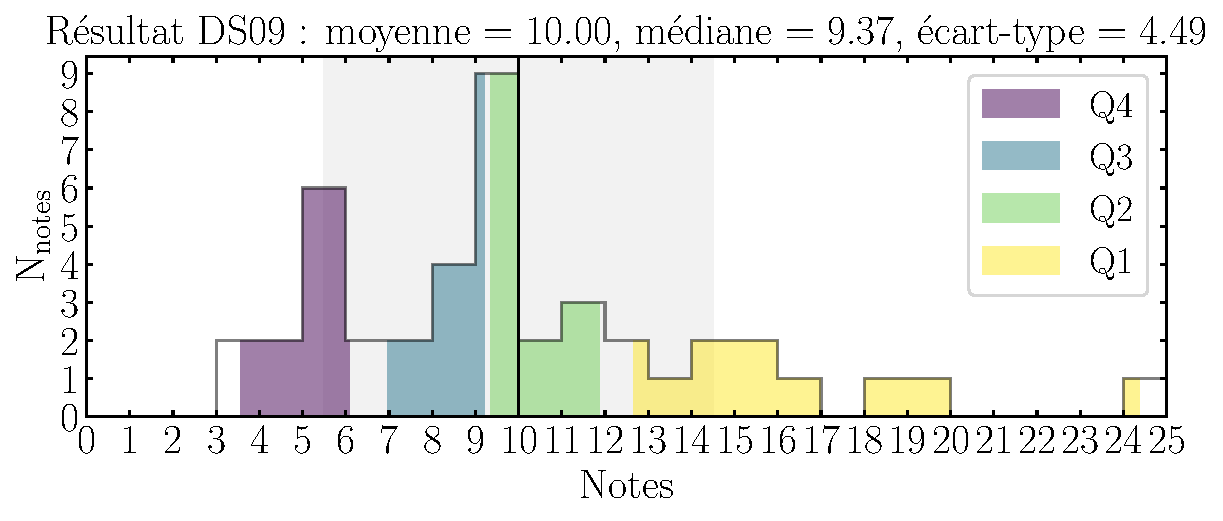
\includegraphics[width=\linewidth]{res_DS09.pdf}
\end{center}
\vspace*{-20pt}

\section{Exercice 1 \hfill \textcolor{red}{/40}}
\begin{enumerate}
	\item Très aléatoire. Pour $T_1$, une compression réduit le volume. Pour
	      $T_2$, diminuer la température diminue le volume à pression constante.
	      \hfill \textcolor{ForestGreen}{/5}
	\item Citez les lois de \textsc{Laplace}. Très bien réussi dans l'ensemble.
	      \hfill \textcolor{ForestGreen}{/8}
	\item Idem.
	      \hfill \textcolor{ForestGreen}{/4}
	\item Quelques variations, sinon très bien. Pensez à citer le 1er principe en
	      entier.
	      \hfill \textcolor{ForestGreen}{/5}
	\item RAS.
	      \hfill \textcolor{ForestGreen}{/5}
	\item $\Delta{U}$ n'est pas nulle que pour un cycle~: sur une isotherme aussi.
	      Encore une fois, adiabatique n'est pas isotherme~!
	      \hfill \textcolor{ForestGreen}{/7}
	\item RAS.
	      \hfill \textcolor{ForestGreen}{/6}
\end{enumerate}

\section{Exercice 2 \hfill \textcolor{red}{/50}}
\begin{enumerate}
	\item RAS.
	      \hfill \textcolor{ForestGreen}{/2}
	\item $\abs{W} =$ aire du cycle.
	      \hfill \textcolor{ForestGreen}{/4}
	\item Toute une variété de courbes, c'est fantastique. Des isothermes
	      concaves, des isochores penchées (trouvez-vous une règle bon sang), des
	      points aléatoires…
	      \hfill \textcolor{ForestGreen}{/5}
	\item Citez \textbf{tout le développement} pour $W$~! Ça n'est pas pour rien
	      que c'est resté en démonstration pendant 4 semaines de khôlles. $P_{\rm ext}
		      \neq P$ si pas réversible ou QS, et $P \neq P_1$~: $V_1$ n'est \textbf{pas}
	      une variable. Pensez également à justifier, par une expression ou la loi de
	      \textsc{Joule}, que $\Delta{U} = 0$ pour une isoT.
	      \hfill \textcolor{ForestGreen}{/12}
	\item RAS de 5 à 7.
	      \hfill \textcolor{ForestGreen}{/4+3+2}
\end{enumerate}
\begin{enumerate}[start=8]
	\item Définir le rendement avant son expression. Pour les moteur, $Q_c$ = tout
	      ce qui est positif.
	      \hfill \textcolor{ForestGreen}{/5}
	\item RAS.
	      \hfill \textcolor{ForestGreen}{/2}
	\item Une rendement de moteur \textbf{ne peut être égal à 1} (et \ul{encore
		      moins l'infini})~!
	      \hfill \textcolor{ForestGreen}{/4}
	\item Quelques bonnes pistes. Faire le lien entre énergie et puissance…
	      ATTENTION~: la température doit \textbf{toujours} être en kelvins.
	      $\frac{T_1}{T_3}$ ne donne pas la même chose en celsius… \hfill
	      \textcolor{ForestGreen}{/7}
\end{enumerate}

\section{Exercice 3 \hfill \textcolor{red}{/56}}
\begin{enumerate}
	\item RAS.
	      \hfill \textcolor{ForestGreen}{/4}
	\item Hypothèse $\ra$ test $\ra$ conclusion.
	      \hfill \textcolor{ForestGreen}{/6}
	\item Pas de théorème des moments sans graphique… il fallait repartir de la
	      source. Négliger $V_L$ devant $V_v$ ne permet pas de négliger $V$ devant
	      $V_V$…
	      \hfill \textcolor{ForestGreen}{/7}
	\item {\Large Vos courbes de rosée doivent être plus penchées~!!} Elle est
	      entre l'isotherme et l'adiabatique. La courbe d'ébullition est pratiquement
	      verticale. Expliquez votre démarche pour la transformation.
	      \hfill \textcolor{ForestGreen}{/8}
	\item Question… très compliquée. Revoir le découpage d'étapes de
	      transformations, en vous appuyant sur le diagramme de \textsc{Clapeyron}.
	      Plein de $\Delta{H}_{\rm calo}$ sortis de nulle part~?
	      \hfill \textcolor{ForestGreen}{/12}
	\item Idem, compliqué. \textbf{Attention}~: $H = U + PV \Ra \Delta{H} =
		      \Delta{U} + \Delta{PV} = \Delta{U} + P \Delta{V} + V \Delta{P}$. Bien penser
	      à la valeur de pression pour un équilibre diphasé vs. vapeur sèche.
	      \hfill \textcolor{ForestGreen}{/12}
	\item Inhomogénéité de $T \Ra$ irréversible $\Ra \Sc_c > 0$.
	      \hfill \textcolor{ForestGreen}{/7}
\end{enumerate}

\section{Exercice 4 \hfill \textcolor{red}{/60}}
\begin{enumerate}
	\item Très peu de points sur une question si simple. N'inversez pas $P
		      \lessgtr P_{\rm sat}$.
	      \hfill \textcolor{ForestGreen}{/1}
	\item Très peu faite, pourtant simple \textsc{Laplace}.
	      \hfill \textcolor{ForestGreen}{/6}
	\item RAS.
	      \hfill \textcolor{ForestGreen}{/4}
	\item Beaucoup de confusion.
	      \hfill \textcolor{ForestGreen}{/7}
	\item Quelques excellentes réponses.
	      \hfill \textcolor{ForestGreen}{/8}
	\item Pareil, revoir le lien entre puissance et énergie, et utiliser à bon
	      escient les unités pour déterminer une relation.
	      \hfill \textcolor{ForestGreen}{/8}
	\item RAS.
	      \hfill \textcolor{ForestGreen}{/6}
	\item Souvent bien, souvent tout confondu. Attention, les éléments physiques
	      (compresseur, etc) ne \textbf{sont} jamais les sources chaudes ou froides,
	      mais sont situés \textbf{au niveau} des sources.
	      \hfill \textcolor{ForestGreen}{/6}
	\item RAS.
	      \hfill \textcolor{ForestGreen}{/4}
	\item[10 et 11)] \textbf{ÉTABLIR} ou \textbf{MONTRER}. Pas de point pour des
		réponses brutes.
		\hfill \textcolor{ForestGreen}{/5+5}
\end{enumerate}

\section{Exercice 5 \hfill \textcolor{red}{/12}}
Exercice à la portée de tout le monde. De bonnes pistes dans l'ensemble, une
seule finalisation. Entraînez-vous à estimer des valeurs du réel.

\end{document}
